\chapter{Introduction}

\begin{figure}[!h]
\centering
            \subfloat[t=0]{
\includegraphics[width=.25\textwidth]{images/glider_gun/1.png}}\hfill
            \subfloat[t=10]{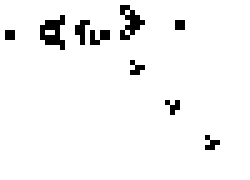
\includegraphics[width=.25\textwidth]{images/glider_gun/2.png}}\hfill
            \subfloat[t=20]{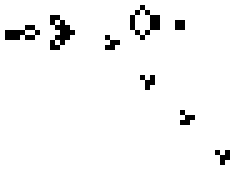
\includegraphics[width=.25\textwidth]{images/glider_gun/3.png}}\hfill
            \subfloat[t=30]{
\includegraphics[width=.25\textwidth]{images/glider_gun/1.png}}\hfill
            \caption{Gosper's Glider Gun, the first known pattern to exhibit unbounded growth in Conway's Game of Life.\cite{hickerson}}
\label{fig:gospers-glider}
\end{figure}

\section{Motivation}
Predicting effects is easier than predicting causes. This is the crux of the Inverse Problem of Science. We find it easier to estimate observations from a parameterised model of the world than to deduce parameters from observations. This results from the causal opacity of time which eliminates information through the unforgiving forces of selection and entropy. Given knowledge of dinosaur evolution, we may have strong hope of predicting where fossils of certain species lie but to build a rigorous taxomony based on fossils alone is insurmountably harder. A physical model of the universe may allow us to predict the subatomic particles ejected when two protons collide at high speed but building theories based on these collisions is significantly more difficult, especially when there are multiple equally valid explanations. Regardless, the pursuit of the Inverse Problem is critical to advancing scientific theory around a system's behaviour. Observations can only validate or falsify but prediction paves the way for novel scientific models.\\

In this thesis, we tackle the inverse problem for cellular automata (CAs). These are simple yet powerful models of computation in which multiple "cells" on a discrete lattice are simultaneously updated at regular time steps. The state of each cell depends exclusively on the state of the cells in a local neighbourhood around it in the previous time step. This localised interaction makes CAs a useful abstract representation of physical and biological systems in the real world from the progression of biological cancer cells\cite{deutsch2021bio, reher2017cell} to the dynamics of urban land use\cite{white2000high}. Much like these systems, CAs can exhibit chaos, nonlinear dynamics, and the emergence of complexity. As well as simulatory models, CAs are powerful computational engines due to their inherently parallel structure. This makes their study a useful endeavour in the field of distributed computation too\cite{tosic2005cellular}.\\

Top-down investigations into CA behaviour are vast and varied[CITE]. Mathematical analyses seek to classify CAs and prove general results about long-term behaviour from intrisic properties. In the natural and social sciences, CAs are designed to model real world systems. Both of these endeavours seek to analyse the behaviour of a CA from its structure, transition function, and initial conditions. In this thesis, we explore a bottom-up approach where we deduce the underlying properties of a CA by observing its behaviour. In particular, we utilise evolutionary algorithms to search across several classes of CA. Evolutionary algorithms (EAs) have long been held as effective tools for black-box optimisation problems. Grounded in the principles of Darwinian evolution, EAs traverse over a search space by performing selection, mutation, and crossover on a population of candidate solutions and increasingly strong solutions are discovered as the fitness of the population increases. Using EAs, we tackle multiple optimisation problems from the imitation of particular CA behaviour to generation of desirable long-term states.\\

\section{Objectives}
We develop a system to discover cellular automata transition functions from observations. We focus on two classes of CA in particular. The first are binary outer-totalistic CA (see \ref{subsec:life-like-ga}) which are the discrete family of models in which Conway's infamous "Game of Life" CA belongs. For this reason, they are also called "Life-like CA". The second are Gray-Scott models which simulate the behaviour of two diffusive chemicals reacting using a continuous vector to represent the density of each chemical in each cell. Key aims of this project include:
\begin{enumerate}
    \item \textbf{Learning Full Rule Dynamics}\label{obj-1}\\
    Deduce the underlying transition rule behind cellular automata of different classes using a broad variety evolutionary computation techniques. Goals includes Life-like CA and Gray-Scott CA. Techniques include genetic algorithms, evolutionary strategies, and particle swarm optimization.
    \item \textbf{Statistical Analysis of Rule Spaces}\\
    Use results from the learning procedures to discover properties of cellular automata that make them more or less predictable. Evaluate how this aligns with existing analyses in the literature.
    \item \textbf{Practical Application of Learning Pipeline}\\
    Using the tools from step~\ref{obj-1} to produce useful solutions to practical optimization problems. This includes the procedural generation of mazes and optimization of transport networks.
\end{enumerate}

\section{Contributions}
The key contributions of this project from a software engineering perspective are as follows:
\begin{enumerate}
    \item \textbf{Evolutionary Algorithm Toolkit}\\ A versatile toolkit that implements multiple evolutionary algorithms to train and optimise different classes of CA. We use this to successfully predict the update rule of life-like CA from observations on random initial conditions. We show that this can be extended to Gray-Scott models where we predict the parameters of diffusion-reaction equations from simulations of chemical reactions.
    \item \textbf{Cellular Automaton Simulator}\\ A system that can efficiently simulate discrete and continuous cellular automata. This allows a broad range of fitness functions to be implemented in the EA toolkit. This can also render snapshots of the CA directly during simulation which allows animations to be efficiently generated afterwards.
    \item \textbf{Procedural Maze Generator}\\ A CA-based maze generation program that uses the EA toolkit to produce difficult mazes with characteristics optimised to user preference.
    
\end{enumerate}
\section{Technical Challenges}